\documentclass[letterpaper,11pt]{article}

\usepackage[margin=1.0in]{geometry}
\usepackage{amsmath}
\usepackage{amsthm}
\usepackage{amsfonts}
\usepackage{algorithm2e}
\usepackage{url}
\usepackage{fancyhdr}
\usepackage{blkarray}
\usepackage{graphicx}
\usepackage{csquotes}
\pagestyle{fancy}
\lhead{Algorithmic-Trading Summary --- Fall 2018}
\rhead{}


\begin{document}
\thispagestyle{plain}
\noindent{Algorithmic-Trading Summary --- Fall 2018}

\noindent{Alex Thomas}

\noindent{Colgate University} \\

\noindent\textbf{Algorithmic-Trading - Summary Paper - Motivations, Foundations, Techniques}

\section*{Introduction and Foundations}

Algorithmic-Trading (AT), is defined as follows: \begin{displayquote} ``In algorithmic trading (AT), computers directly interface with trading platforms, placing orders without immediate human intervention. The computers observe market data and possibly other information at very high frequency, and, based on a
built-in algorithm, send back trading instructions, often within milliseconds. A
variety of algorithms are used: for example, some look for arbitrage opportunities,
including small discrepancies in the exchange rates between three currencies; some
seek optimal execution of large orders at the minimum cost; and some seek to
implement longer-term trading strategies in search of profits.'' (Chaboud et al.
2009). \end{displayquote} In other words, AT is the generation and submission of buy and sell orders by an algorithm, or set of instructions that processes current market data and places orders in stock marketplaces without human interaction. 

High Frequency Trading (HFT), is a subset of algorithmic trading and a far newer phenomenon that has been made possible by the rapid improvement of computerized trading speed. This is the primary form of algorithmic trading found in financial markets today, with billions of dollars constantly traded by machines every second. 

AT is largely unregulated. There are absolutely no restrictions on electronic trading, which has resulted in various performance throughout entire markets. See the Flash Crash below. Especially with the rise of costless transactions with platforms like Robinhood, it has never been easier for individuals to engage in AT. 

Rapid trading traces its roots back to the early 1930s, with specialists and pit traders buying and selling positions at a physical location of the exchange and broadcasting it via telegram services.  Computerization of trades started in the 1980s when the NASDAQ introduced purely electronic trading. Today, HFT trading time has changed from a matter of seconds to microseconds. 

The May 6th, 2010 "Flash Crash" brought the public's attention to the little publicized, but very heavily used algorithmic trading in financial markets. This happened with E-mini, denoted by ES, which is a stock market index futures contract that trades for around 50 times the value of the S\&P. A mutual fund complex sold 75,000 of these contracts valued at approximately $4.1$ billion dollars - resulting in the largest net change in daily position of any trader in the E-mini since the beginning of the year. This caused a cascading effect, although initially absorbed by HFT's, with over 20,000 trades across 300 separate securities executing at prices 60 percent away from their prices a mere half hour earlier.  

\subsection*{Motivations for Research}

AT is a relatively secretive area of financial trading, but can result in massive profits if performed correctly with proper portfolio management, risk and alpha models. 

\section*{Key Techniques}

\begin{figure}[ht!]
\centering
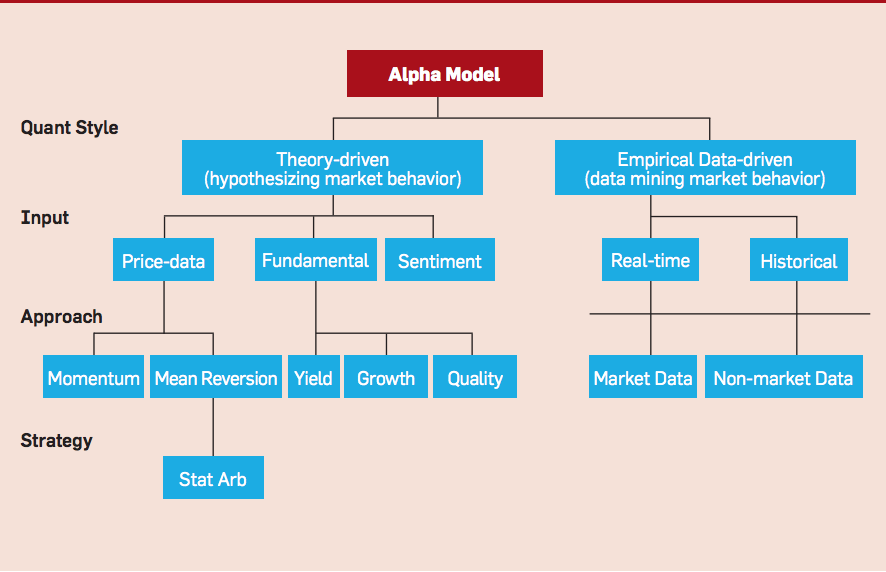
\includegraphics[width=90mm]{alpha.png}
\caption{Alpha Models \label{overflow}}
\end{figure}

\subsection*{Simple Moving Average (SMA)}

(see Teixiera, Oliveria for mathematical representation)

This is calculated by adding a certain amount of closing prices and dividing by the total amount of days. Short term averages are often compared against longer term averages, often signaling uptrends and downtrends. Popular methods include the golden cross and death cross, with the 50 day SMA crosses below or above the 200 day moving average. The former is often a buy signal reinforced by high trading volumes while the latter is considered bearish.
\subsection*{Pairs Trading and Arbitrage}

Statistical arbitrage uses time series methods to identify brief pricing errors of stocks. HFT takes advantage of this because these discrepancies in price exist for mere fractions of a second. Statistical arbitrage is something that is far more practical to implement in the bitcoin market, especially without the tools that prop-trading firms have. Pairs trading uses arbitrage by choosing stocks that are correlated and move similarly. 

\subsection*{Market Making}

Another common form of algorithmic trading often used by large funds or market makers in a financial market. It provides both advantages to the market making institution as well as the market participants. Automated scripts will never deviate into risky actions that human traders may complete and further reduces the incidence of market crashes and negative surprises for the market maker's bottom line. A sample naive market making strategy is fixed offset, which continuously places limit orders on both sides a specified number of ticks away from the market price.

\subsection*{Mean Reversion}

This strategy assumes that prices and returns eventually move back towards the mean. Pairs trading takes advantage of this by choosing stocks that are historically correlated that have diverged and will most likely converge in the future. 

\subsection*{Machine Learning - Bayesian networks}

A bayesian network is a dag that represents a set of variables and their conditional dependencies. In this case, it will give decisions based on certain market conditions and prices to sell or buy a particular stock based on this learned conditional dependencies. Interesting research suggests that gated bayesian networks are far more effective in AT. 

\subsection*{Momentum Trading Strategies}

General strategies that aim at capturing trends in the market fall under this umbrella. SMA is an example of a momentum trading strategy. 

\subsection*{Risk Model}

This method is less of a trading strategy and more of a stop method used to evaluate portfolios. A sample model may evaluate the VAR (value at risk) for everything owned in the portfolio. If the VAR reaches a certain threshold in comparison to its value, close all positions in the portfolio. 

\subsection*{Bollinger Bands}

These are designed to compare volatility and relative price levels over time. There are 3 measures or "bands", with a SMA in the middle accompanied by two bands above and below which are SMA $+/-$ a given number of standard deviations

\subsection*{RSI - Relative Strength Index}

This is one of the most popular momentum oscillators and compares the magnitude of recent gains to the magnitude of recent losses and gives a number between 0 and 100. When it falls below 70 it is considered a bearish signal while if it's above 30 that is generally a bullish signal. The equation is given as RSI $= 100 - (100/(1+$avgGain$/$avgLoss$))$

\section*{Conclusion}

AT and HFT are far more secretive than I would have imagined. With the expansion of financial literacy and wide tools available today to trade over nearly every market now available to the average person, I would have expected a far more open-source, collaborative community that you find in the software/computer science field. 

SMA and its application with the dual moving average strategy is a simple and naive AT strategy. However, many applications such as EMA and Bollinger Bands use moving average as its basis. Pairs trading and arbitrage strategies are much more involved. Other models and metrics such as VAR give a different side of AT that is more focused on portfolio management and risk.

\bibliographystyle{plain}
\nocite{*}
\bibliography{References}


\end{document}